\section{Background}

The shape-and-effect inference system described by Abal et. al. \cite{Abal2017EffectiveBF} enables \textit{"[...] efficient and scalable inter-procedural reasoning about resource manipulation"}. Abal et. al. describe a method for detecting double-lock bugs in the kernel source code using the shape-and-effect system in the EBA analyzer.

\newpar The same shape-and-effect analysis can be used to build more error checker. Extending the existing implementation allows building another error checker relatively fast, since the implementation is already able to run on the Linux kernel components.

\newpar The Linux kernel source code can be analyzed using existing static analysis tools in order to build a Control Flow Graph (CFG) of a given kernel component implementation. The control flow graph shows the possible execution paths of the component. )One can then formulate Computational Tree Logic to sepcify desirable and undesirable execution paths (errors). 

\newpar The following example shows how to formulate the double \textit{lock} error using CTL: 

\begin{center}
    $\top\:\mathrm{EU}\:\left({l o c k}_{\rho} \wedge\:\mathrm{EX}\:\left(\neg {u n l o c k}_{\rho}\:\mathrm{EU}\:{l o c k}_{\rho}\right)\right)$
\end{center}

\newpar This example states that I am interested in finding a double lock locking the same memory region $p$. The formula describes execution traces in which, after a prefix, a lock is taken on $p$ and a second lock is eventually taken on $p$ without an unlock on $p$ in between the two locks. This CTL formulation can be visualized as seen in Fig \ref{fig:doublelock}.

\begin{figure}[h]
    \centering
    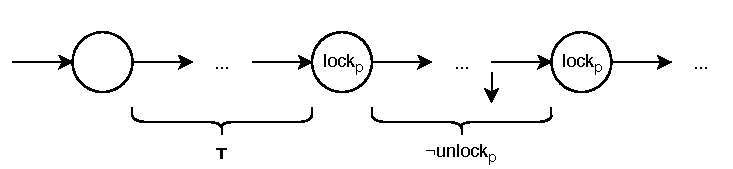
\includegraphics{background/figures/doublelock}
    \caption{The CTL form of a double lock error visualized.}
    \label{fig:doublelock}
\end{figure}

\newpar Computation tree logic models program executions in time as tree-like structures where all paths can be the actual path executed at runtime. The specifics of the CTL formulation is not the focus of this project, instead the CTL notation is merely used to formalize which errors I want to find in the Linux kernel source code --- in this case a double-unlock error.

\newpar The inverse problem --- the case of two unlocks being present with no locks in between them --- can therefore be formulated in CTL as: 

\begin{center}
    $\top\:\mathrm{EU}\:\left({u n l o c k}_{\rho} \wedge\:\mathrm{EX}\:\left(\neg {l o c k}_{\rho}\:\mathrm{EU}\:{u n l o c k}_{\rho}\right)\right)$
\end{center}

\newpar The formula describes execution traces in which, after a prefix, an unlock is performed on $p$ and a second unlock is eventually performed on $p$ without a lock taken on $p$ in between the two unlocks. I am interested in finding a double unlock locking the same memory region, since this is where the undefined behaviour would occur. The visualization of this can be seen in Fig \ref{fig:doubleunlock}.

\begin{figure}[h]
    \centering
    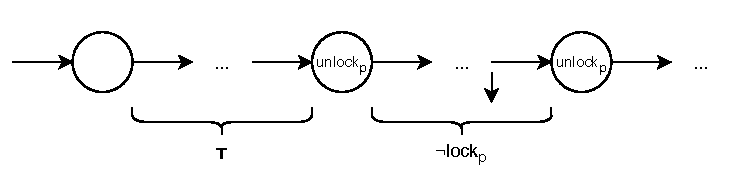
\includegraphics{background/figures/doubleunlock}
    \caption{The CTL form of a double unlock error visualized.}
    \label{fig:doubleunlock}
\end{figure}

\newpar The existing implementation of the EBA analyzer explores the CFG of the Linux kernel while checking on the fly that a given undesired execution path is not present in the source code. If such an execution path is found, a bug is possibly present in the analyzed component, and an error is raised.

\newpar The implementation of the EBA analyzer uses a concept of \textit{may lock} and \textit{must lock} internally similar to the concept described by Godefroid et. al. \cite{Godefroid}. A lock within an \texttt{if} statement on a dynamic value is represented as a \textit{may lock}, since it is uncertain whether the \texttt{if} statement will evaluate to \texttt{true} at runtime. On the other hand, a \textit{must lock} is an explicit lock within the code which will always be executed. This concept of \textit{may} and \textit{must} also applies to the double unlock problem, where a \textit{may unlock} is an unlock in an execution branch which might not be executed at runtime. A \textit{must unlock} is an explicit unlock where a lock will always be unlocked at runtime.

\newpar The implementation of the EBA analyzer supports implementing separate error checkers in a plug-and-play nature. This allows implementing a double unlock checker as a separate module in the implementation source code and making this available to the user(s) of the analyzer using a command-line parameter. The following section will elaborate on the implementation details of my work which has been integrated into the EBA code base in this manner. 